\chapter{Presentation of the new test network}




\section{Goals for the new testbed}


The main goals for the new testbed are the following:
\begin{itemize}
	\item A test network as close as possible to a real life situation
	\item Possibility to remotely supervise both the Wi-Fi and UHF (Ultra High Frequency) communications
	\item Easy to use
	\item	Easy to reproduce elsewhere
	\item Affordable
	\item Easy to expand
\end{itemize}

This is a list of the features I was aiming for in this project. 
The network should be as close as possible to a real life situation. Indeed, if we want to test the Mesh Extenders, it is better to test them in a coherent scenario. We want them to be far enough from each other, so they don't rely only on Wi-Fi. We want them to be connected to other devices who can use the Serval network (phones for example). Obviously we will never have a true real situation since we are locked in the building and cannot set-up the network outside of the building. We are also limited in the number of devices at our disposal. These two points are limitation we have to work with.

We want the network to be practical. In the current testbed, we have to move around the build between the sites to test it. In the new testbed, we should be able to test everything from the lab.

The new test network should be easy to use and reproduce. The team in the Lab are obviously expert on the Serval project and could work with a very particular test network. However, this network could be reproduced by other teams who want to work on the project. They may not be too familiar with the project at the beginning, but they will probably still want to use the test network. That's why it should be easy to use (should be user friendly and be well documented) and easy to reproduce (thanks to a good documentation). 

We want the test network to be affordable. The first reason for this is linked to the previous point. Indeed, if we want other people to be able to recreate the test network, it should be as least expensive as possible. Indeed, they may not have access to a lot of funds or may not want to spend too much money (they could work on the project as a tech enthusiast).
The second reason is the budget of the team. 

Finally, the testbed should be easy to expand. The team is still working on the Serval project, improving it and adding new functionalities. Therefore, the testbed may have to evolve to test these new features. 

All these wanted properties and the environment we are working with create constraints and challenges we have to deal with or overcome.


%%%%%%%%%%%%%%%%%%%%%%%%%%%%%%%%%%%%%%%%%%%%%%%%%%%
%								Next Section 											%
%%%%%%%%%%%%%%%%%%%%%%%%%%%%%%%%%%%%%%%%%%%%%%%%%%%

\section{Constraints and challenges}


There are a lot of constraints we need to work with.

The first constraint is the environment we are working with. Indeed, Mesh Extenders are designed to be far from each other. But here, we are setting up a test network inside a building. That means we need to check how the Mesh Extenders are connecting to each other. We want to make sure they are using UHF to connect to other Mesh Extenders. It will limit the number of Mesh Extenders we can use in the test network. Right now, we want to use only 4 Mesh Extenders, so it is still manageable.

The Mesh Extenders being close create another issue. We would like to be able to test them when the signal is low to see how they handle package errors. "Thankfully", the walls in the building are quite good at blocking radio signal. Therefore, with the basic set-up Paul noticed that the UHF signal between the Mesh Extender on the first floor and one Mesh Extender on the fourth floor was very low. He even had to put a better antenna to the Mesh Extender on the first floor to improve the signal.

The last constraint is time. The available time for the project is very short. Indeed, the project was started after the mid semester break at the end of April/ beginning of May. Therefore, I had two months to make it.

Constraints are imposed by your environment, your possibilities whereas challenges are imposed by yourself. For this project, the properties of the test network are creating many challenges.

First our budget is limited. We want an affordable solution. Therefore, we decided to limit the budget for this project to the amount given by Flinders for the master project. It means that we have around 300 dollars to buy the needed device. Thankfully some of them were already in the Lab (the Mesh Extenders, cables, and the RFD900+). This budget means we don't have access to every solutions possible. Therefore, I had to work with limited devices and find work around.



Keeping in mind all these constraints and challenges, I came up with a design for the test network. 




%%%%%%%%%%%%%%%%%%%%%%%%%%%%%%%%%%%%%%%%%%%%%%%%%%%
%								Next Section 											%
%%%%%%%%%%%%%%%%%%%%%%%%%%%%%%%%%%%%%%%%%%%%%%%%%%%



\section{Design of the new testbed}


For the new test network, we will still have 4 sites at different places in the building. However, on each site, there will be more than just a Mesh Extender.

On each site we will find:
\begin{itemize}
	\item a Mesh Extender
	\item a small linux router
	\item an android phone
	\item a usb hub
	\item a RFD900+
\end{itemize}


In addition to this 4 sites, we add an additional set-up in the Telecommunication Lab. It will be the access point to the test network.

\subsection{Hardware used for the testbed}

First, for this test network, we will obviously need Mesh Extenders:
\begin{figure}[H]
\begin{center}
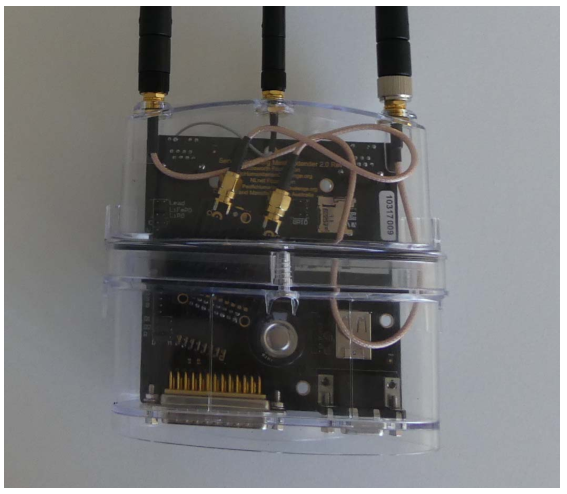
\includegraphics[width=8cm]{image/meshextender.png}%
\caption{Mesh Extender}%
\label{figure:ME}%-
\end{center}
\end{figure}


In this project we are also using small Linux routers to built the network we will use to supervise the Mesh Extenders.

The small routers we have chose to use are: the GL-AR150 and GL-AR750.

\begin{figure}[H]
\centering
\begin{subfigure}{.5\textwidth}
  \centering
	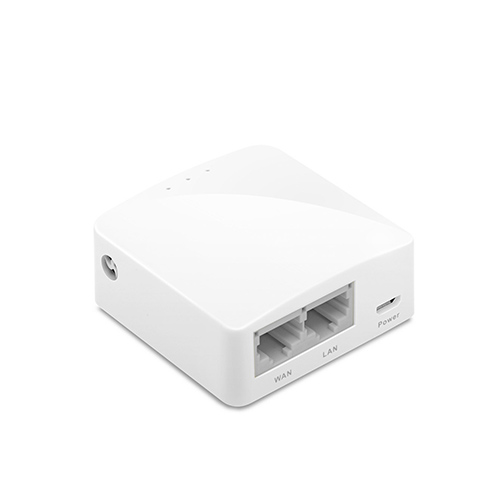
\includegraphics[width=8cm]{image/AR150.jpg}%
	\caption{GL-AR150}%
	\label{figure:AR150}%-
\end{subfigure}%
\begin{subfigure}{.5\textwidth}
  \centering
  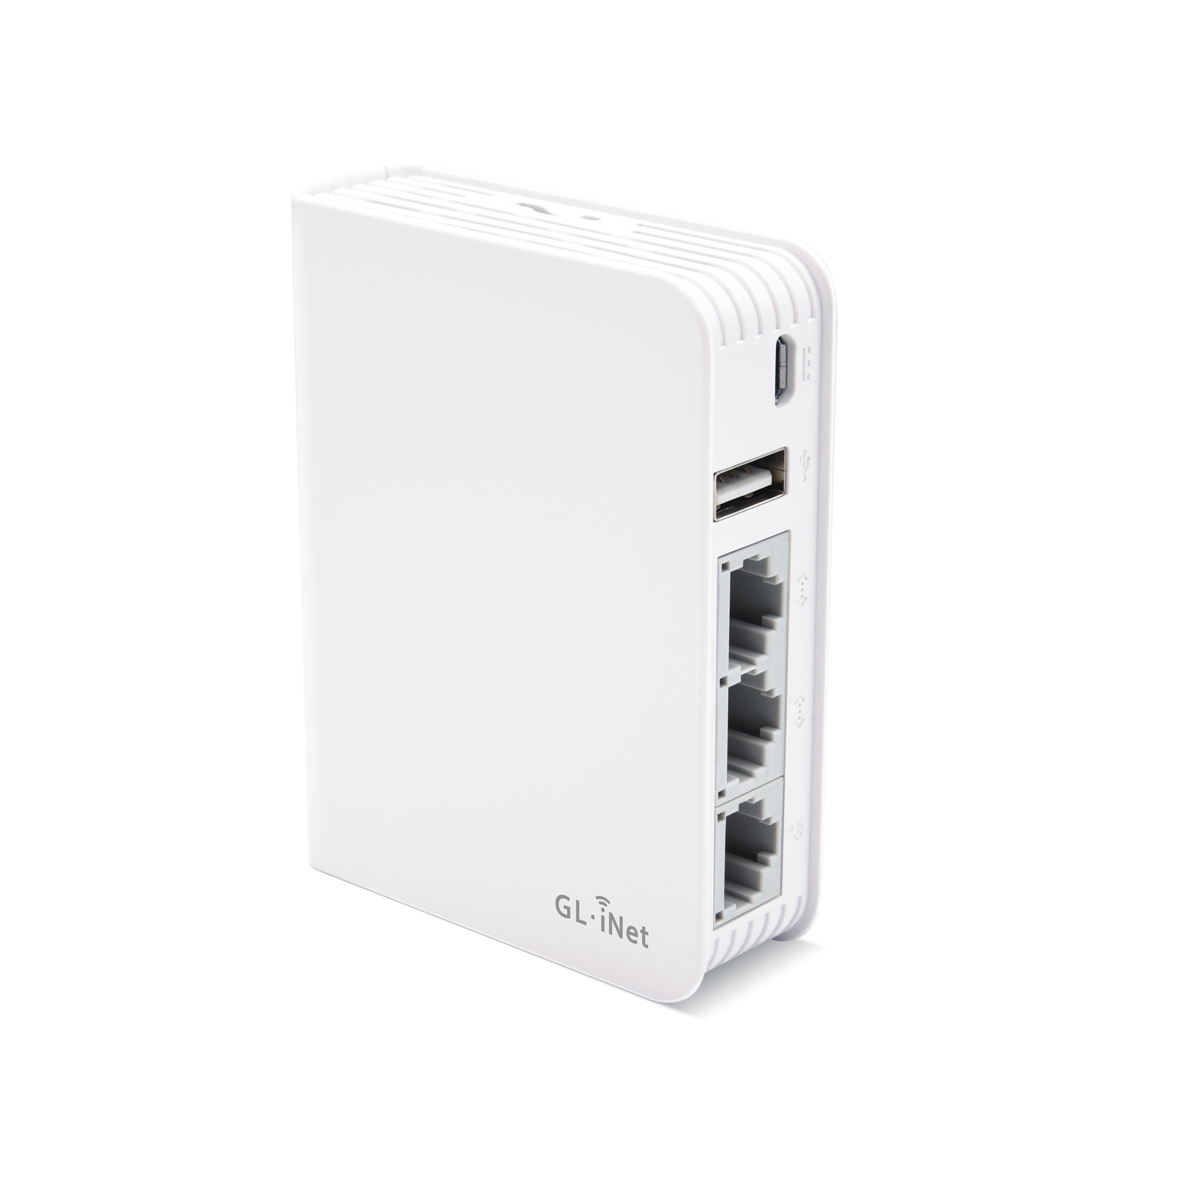
\includegraphics[width=8cm]{image/AR750.jpg}%
	\caption{GL-AR750}%
	\label{figure:AR750}%-
\end{subfigure}
\caption{Routers used for the testbed (source: https://www.gl-inet.com/)}
\label{fig:routers}
\end{figure}


These two routers are great for the test network. Indeed, they are small, affordable and we have a lot of freedom since their OS is based on a Linux kernel (the OS used for the Mesh extenders can also be put inside these routers).
The only issue we can have is the fact they do not have a lot of USB ports and no UHF radio. Therefore we need other devices:
\begin{figure}[H]
\centering
\begin{subfigure}{.5\textwidth}
  \centering
	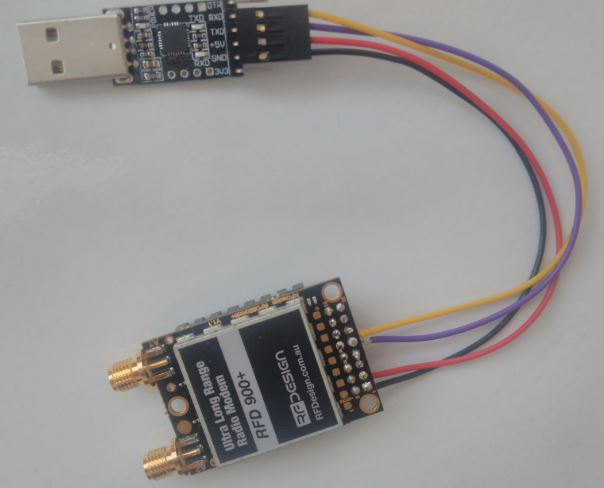
\includegraphics[width=8cm]{image/rfd900.jpg}%
	\caption{RFD900 with a serial to USB adapter}%
	\label{figure:RFD900}%-
\end{subfigure}%
\begin{subfigure}{.5\textwidth}
  \centering
  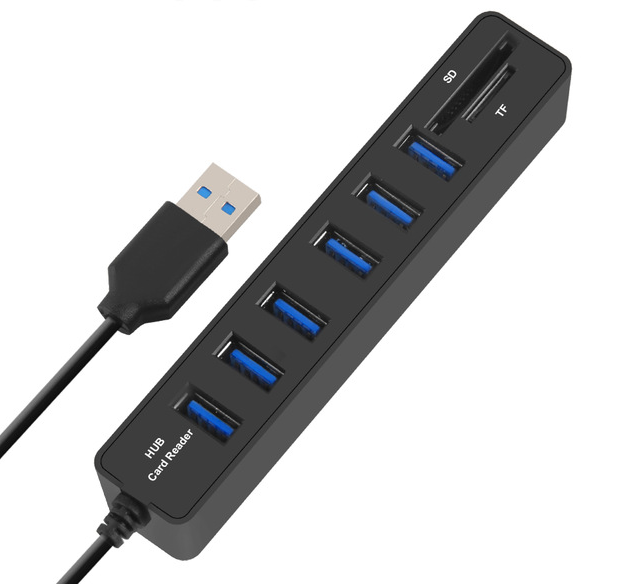
\includegraphics[width=8cm]{image/usbhub.jpg}%
	\caption{USB hub}%
	\label{figure:UsbHub}%-
\end{subfigure}
\caption{Other devices needed}
\label{fig:devices}
\end{figure}

To monitor the UHF packets of the Mesh Extenders, we need a RFD900+. Since the RFD900+ has a serial interface (pins), we need to create an adapter to plug it using USB.
We are using a USB hub to increase the number of USB ports on the router.

We now have all the needed hardware.





\subsection{Big picture}

As explained previously, there are two types of site in this test network:
\begin{itemize}
	\item The remotes sites where the Mesh Extenders are
	\item The main site used to interconnect the remotes sites and act as an access point
\end{itemize}

%figure main site








%figure remote site


\subsubsection{Global design of the network}

To interconnect them, we need to design a network solution.
I have come up with the following solution:
\begin{figure}[H]
\begin{center}
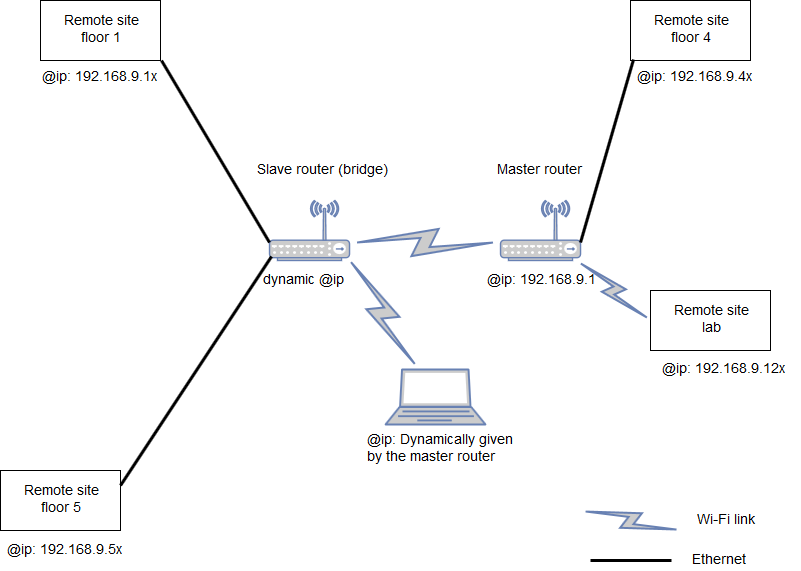
\includegraphics[width=\textwidth]{image/networkBigpicture.png}%
\caption{Big picture of the network}%
\label{figure:NetworkBigPicture}%-
\end{center}
\end{figure}

Since we want to be able to communicate with all the devices from the laboratory, the easiest solution is to create only one network. All the devices are in the same network and no routing is needed. The main router is an access point to the network and every communication has to go through it. Therefore, we have one point where we can control the network. These properties are very important. Indeed, since they are all in the same network, each device should be able to communicate with another through this network. It means that a Mesh Extender could use this network to send a message to another Mesh Extender using this network. However, since all communications have to go through the main router, we can avoid this situation. Indeed, we can set rules in the main router to prohibit communication between remote sites.

Another important point of this design is the distribution of IP addresses. The slave router and all the computers connected to this network will receive dynamic IP addresses. However, the remote sites will have fixed addresses for three reasons:
\begin{itemize}
	\item First, the remote servers need fixed hostnames for my software solution. By giving fixed IP addresses, the main router can also assign them a hostname
	\item The second reason is linked to the issue explained earlier. If they have fixed addresses, it will be easier to add traffic rules for these devices
	\item Finally it is easier to recognise each remote device is if they have fixed addresses.
\end{itemize}

In this design, the slave router is simply a bridge that extends the main router. GL-AR750 can be configured as bridges but only if they are linked with Ethernet. However, in my design, they are communicating by Wi-Fi. Luckily, we can simulate this bridge behaviour using a Linux packet called relayd.




\subsubsection{Global design of the software}

In this project, we are going to use C programs to remotely supervise the Mesh Extenders.
C language was chosen because:
\begin{itemize}
	\item It is a light and efficient language (which is great since our routers don't have a lot of power or memory)
	\item In the Serval project most of the coding was made in C. We can easily integrate other parts of the Serval project inside the test network.
\end{itemize}


I have decide to create a TCP client-server system composed of 3 files:
\begin{itemize}
	\item server.c which will be on the small routers
	\item client\_shell.c and client.c which will be for the user
\end{itemize}

I will explain what each file does in the next section.


A TCP client-server was not the only solution. However, I still opted for it because:
\begin{itemize}
	\item I was more used to code a TCP server and client than other solutions. Therefore, I will be faster using this solution.
	\item The libraries for TCP are quite old and should work on most devices.
\end{itemize}


The software part corresponds to the communication between a few programs:
\begin{itemize}
	\item The client\_shell and the client
	\item The client and the server
	\item The server and the RFD900+
\end{itemize}

For the communication between the server and the RFD900+, we use the driver in C developed by Paul. This part use the code of the LBARD git repository.

\hfill \break

We want to establish the following communication process:
\begin{figure}[H]
\begin{center}
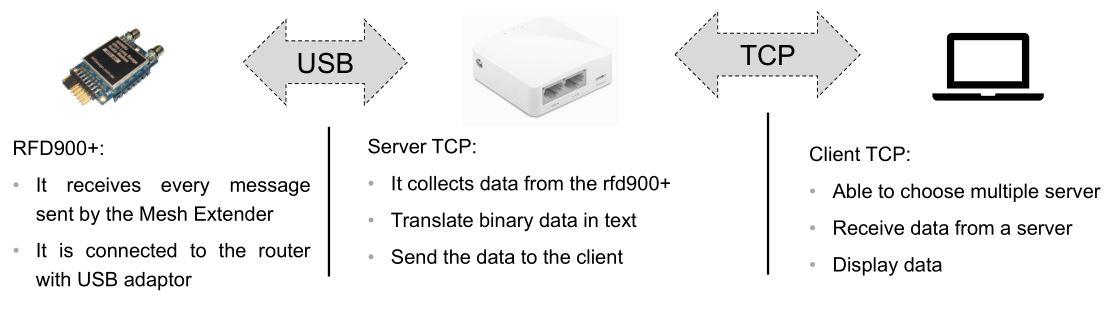
\includegraphics[width=\textwidth]{image/GlobalUHF.jpg}%
\caption{Mesh Extender's messages through the testbed}%
\label{figure:UHFmesh}%-
\end{center}
\end{figure}

\hfill \break



\hfill \break \underline{\large{\textbf{Communication between the server and the client}}}

The communication between the client and the server is very basic. Most of the time the client is only receiving packets from the server and displaying them on the computer.

But the client can also send a few messages to the server. These messages allow the client to close the communication with the server. Later they will also allow the client to change what is supervised.

\begin{figure}[H]
\begin{center}
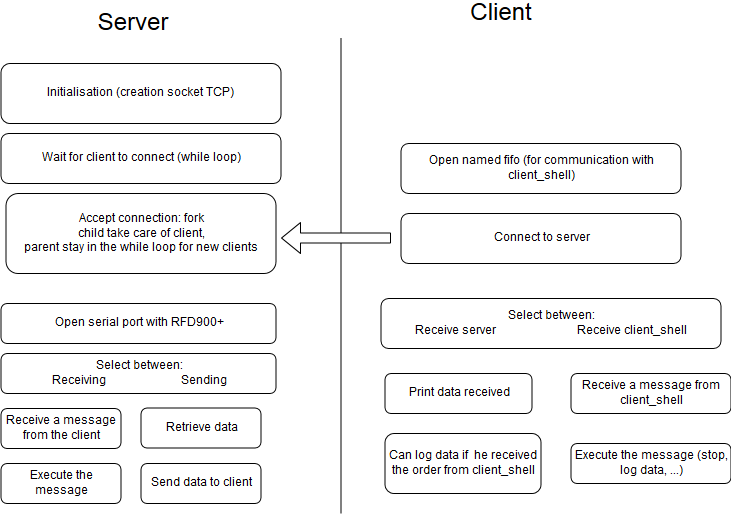
\includegraphics[width=\textwidth]{image/clientServer.png}%
\caption{Client and server communication}%
\label{figure:CS}%-
\end{center}
\end{figure}

The server start as a classic TCP server. It will create the socket for the server (a socket is basically the combination of source and destination IP address and port). Then it will listen on the socket to see if a client is trying to connect. Each time the server receive the connection, he starts a process to handle the client and keeps listening for new client. The process that handles the client work in a loop. In the loop, the process start by looking if the client sent a message. If he received a message from the client, the server analyses the message and execute the corresponding code. The messages can be used to stop the connection or change the behaviour of the server (what we want to supervise for instance). If the process does not receive a message from the client, it will send data to the client. By default, the data are the UHF packets sent by the Mesh Extenders.


\hfill \break \underline{\large{\textbf{Interactions between the client\_shell and the client}}}

The client\_shell is a shell-like interface that gives access to all the available functionalities.
It can:
\begin{itemize}
	\item Find the available servers using a file containing the hostnames of servers
	\item Launch a client
	\item Communicate with the client to send different orders such as
		\subitem "`STOP"' to close the connection
		\subitem "`LOG Filename"' to start logging the data
  \item Keep a list of all the current clients created
	\end{itemize}




\begin{figure}[H]
\begin{center}
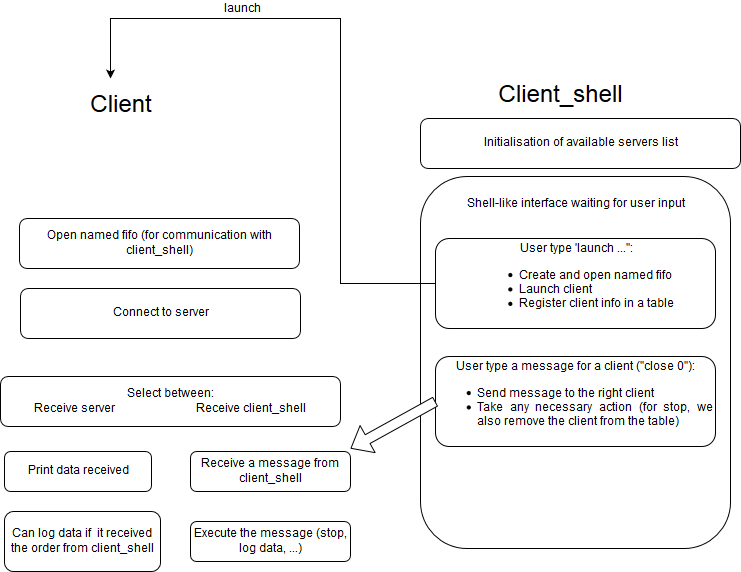
\includegraphics[width=\textwidth]{image/clientshellClient.png}%
\caption{Client and Client\_shell interaction}%
\label{figure:CSC}%-
\end{center}
\end{figure}



The client\_shell is a shell-like interface. It will start by initialising the list of server available. Using a file containing all the possible servers’ name, it will try to find which servers on the list is available at the moment. Then, it will wait for an input of the user.
The available commands are:
\begin{itemize}
	\item help: list the available built in functions
	\item exit: close the client\_shell
	\item launch: launch a client
	\item findServers: update the list of available servers
	\item displayServers: display the available servers
	\item close: close a client
	\item list: list the clients currently running 
	\item log: start or stop logging the data for one client
\end{itemize}

If you type a function but do not put the right parameters, the shell will display a short message
explaining how to use the function properly.


The client starts by opening the named FIFO (First In First Out: a pile of messages where they are read and written in the same order) that was created by the client\_shell. The client will receive order of the user through this named FIFO. Then the client will connect to the server. Once connected it will see if he received a message from the server or the client\_shell.
If he receives a message from the server, it will display it, and he can logged it if the user wants to.
If he receives a message from the client\_shell, it will understand the order and execute it. The order can be to log the data received from the server in a file or to close the connection with the server for example.

The client can be manually started by a user. In this case, the client will read the input from the client using the standard input. If the user type "STOP" in the shell where he started the client, it will close the connection with the server. Using the client this way is harder because you need to know exactly what to type to send an order to the client, and the client is constantly displaying text on the screen making it hard to type.


